% ---
% school: "college"
% level: "8eme"
% section: null
% chapter: "التناظر المركزي"
% source: "Axiomaths"
% title: "متوازي أضلاع ومنتصفان"
% country: "Tunisie"
% year: 2026
% professor: "Axiomaths"
% difficulty: "Moyen"
% points: null
% tags: ["symetrie-centrale", "parallelogramme", "milieu", "diagonales"]
% ---
% Exercice 6/15 de la série 8ème « التناظر المركزي » (statement + \axsol + solution). Compiler avec XeLaTeX + axiomath.sty (+ axiomaths-logo.png).
\documentclass[12pt,a4paper]{article}
\usepackage[level=8b,color=15803D]{axiomath}
\usetikzlibrary{arrows.meta}
\newcommand{\cm}{\,\mathrm{cm}}
\axsetup{title={التناظر المركزي}, corrige}

\begin{document}

\begin{corr}[title={متوازي أضلاع ومنتصفان}, stars=3, source={Axiomaths}]
$ABCD$ متوازي أضلاع مركزه $O$ (نقطة تقاطع قطريه) و $E$ منتصف $[AB]$.
\begin{center}
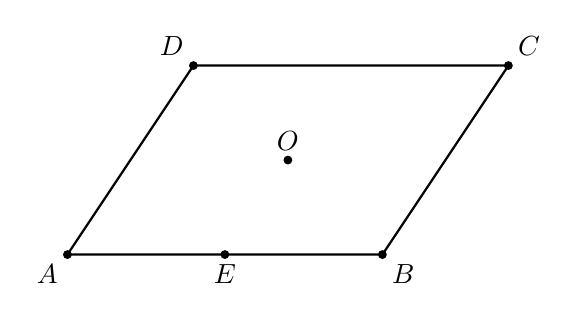
\begin{tikzpicture}[scale=0.8]
  \draw[thick] (0,0)--(5,0)--(7,3)--(2,3)--cycle;
  \fill (0,0) circle (2pt) node[below left] {$A$};
  \fill (5,0) circle (2pt) node[below right] {$B$};
  \fill (7,3) circle (2pt) node[above right] {$C$};
  \fill (2,3) circle (2pt) node[above left] {$D$};
  \fill (3.5,1.5) circle (2pt) node[above] {$O$};
  \fill (2.5,0) circle (2pt) node[below] {$E$};
\end{tikzpicture}
\end{center}
\begin{enumerate}
  \item ما هما مناظرا $A$ و $B$ بالنسبة إلى $O$ ؟
  \item $F$ مناظرة $E$ بالنسبة إلى $O$. بين أن $F$ منتصف $[CD]$.
  \item بين أن $AECF$ متوازي أضلاع.
  \item استنتج أن $(EC)\parallel(AF)$ ، ثم بين أن $(BF)\parallel(ED)$.
\end{enumerate}
\axsol
\begin{enumerate}[itemsep=14pt]
  \item\leavevmode
  \begin{prop}[قطرا متوازي الأضلاع]
  قطرا متوازي الأضلاع يتقاطعان في منتصفهما : \ib{$O$ منتصف $[AC]$ و $[BD]$}.
  \end{prop}
  إذن مناظرة $A$ هي $C$ ومناظرة $B$ هي $D$.
  \item $S_O$ يحوّل $A$ إلى $C$ و $B$ إلى $D$ ، فمناظر $[AB]$ هو $[CD]$. والتناظر المركزي يحفظ المنتصفات : مناظر $E$ (منتصف $[AB]$) هو منتصف $[CD]$. إذن $F$ منتصف $[CD]$.
  \item للرباعي $AECF$ القطران $[AC]$ و $[EF]$. $O$ منتصف $[AC]$ ، و $O$ منتصف $[EF]$ لأن $F=S_O(E)$. القطران لهما نفس المنتصف، إذن $AECF$ \ib{متوازي أضلاع}.
  \begin{center}
  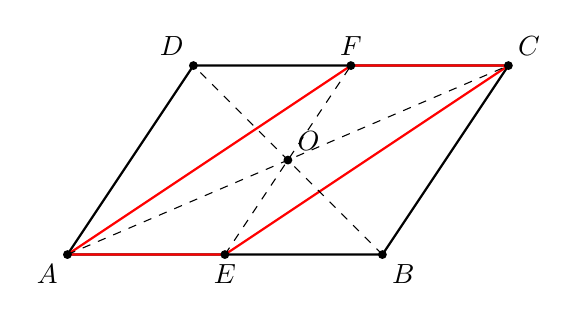
\begin{tikzpicture}[scale=0.8]
    \draw[thick] (0,0)--(5,0)--(7,3)--(2,3)--cycle;
    \draw[red,thick] (0,0)--(2.5,0)--(7,3)--(4.5,3)--cycle;
    \draw[dashed] (2.5,0)--(4.5,3);
    \draw[dashed] (0,0)--(7,3);
    \draw[dashed] (5,0)--(2,3);
    \fill (0,0) circle (2pt) node[below left] {$A$};
    \fill (5,0) circle (2pt) node[below right] {$B$};
    \fill (7,3) circle (2pt) node[above right] {$C$};
    \fill (2,3) circle (2pt) node[above left] {$D$};
    \fill (3.5,1.5) circle (2pt) node[above right] {$O$};
    \fill (2.5,0) circle (2pt) node[below] {$E$};
    \fill (4.5,3) circle (2pt) node[above] {$F$};
  \end{tikzpicture}
  \end{center}
  \item في متوازي الأضلاع $AECF$ الضلعان $[EC]$ و $[AF]$ متقابلان، إذن $(EC)\parallel(AF)$.
  وللرباعي $EBFD$ القطران $[EF]$ و $[BD]$ لهما نفس المنتصف $O$ ، فهو متوازي أضلاع ومنه $(BF)\parallel(ED)$.
\end{enumerate}
\end{corr}

\end{document}
